\chapter{Технологическая часть}

\section{Общая архитектура системы}

\subsection{Процесс обработки данных}

Независимо от того, какой именно математический метод будет осуществлять позиционирование устройства на основе имеющихся данных, можно с уверенностью сказать, что в системе будут поочерёдно или параллельно происходить два процесса: обучение и использование.

Процесс обучения состоит из следующих этапов:

\begin{enumerate}
	\item
		Измерение RSSI видимых базовых станций устройством, оборудованным модулем спутниковой навигации;
	\item
		Передача данных о базовых станциях и положении устройства на сервер;
	\item
		Приём и первоначальная обработка данных сервером. В этот этап могут входить такие процессы как проверка корректности, преобразование координат из пары широта/долгота в пару маршрут/расстояние и так далее;
	\item
		Сохранение собранной информации в базе данных;
	\item
		После набора достаточного количества данных --- вычисление необходимых данных для алгоритма позиционирования (обучение).
\end{enumerate}

Процесс позиционирования проходит следующим образом:

\begin{enumerate}
	\item
		Измерение RSSI видимых базовых станций устройством, не оборудованным модулем спутниковой навигации;
	\item
		Приём данных сервером;
	\item
		Вычисление предполагаемого расположения устройства с помощью обученного алгоритма;
	\item
		Если требуется --- обратное преобразование координат в двухмерные (например, для отображения на карте), хотя этот шаг может и отсутствовать (так, для электронного табло на остановке более подходит именно расстояние по маршруту);
	\item
		Передача данных о положении устройства клиентам.
\end{enumerate}

\subsection{Состав системы}
На основании данного описания логики работы системы, предложена архитектура, изображённая на рис. \ref{fig:general-arch}.

\begin{figure}[h]
	\center{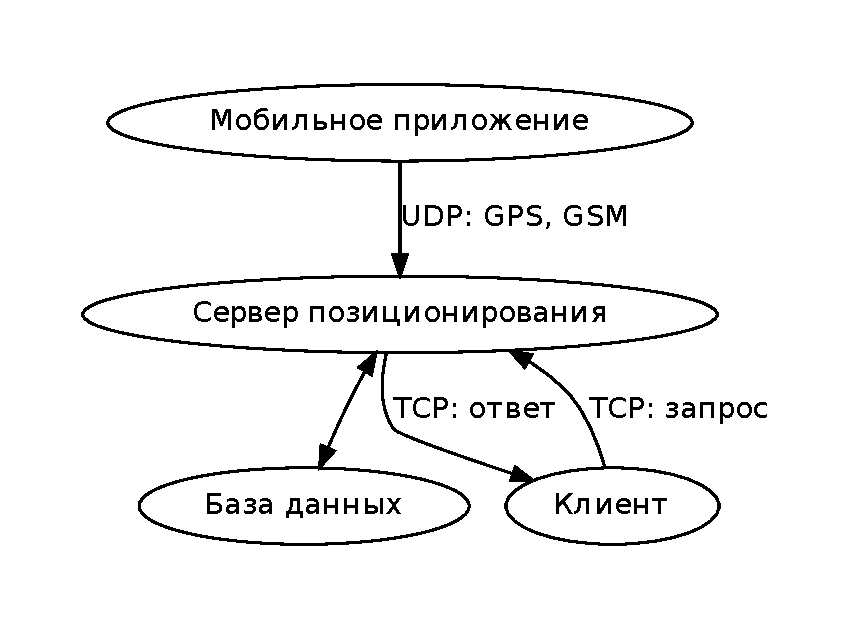
\includegraphics[width=1\linewidth]{general-arch.pdf}}
	\caption{Общая архитектура разрабатываемой системы}
	\label{fig:general-arch}
\end{figure}

Приложение, работающее на мобильном устройстве, в зависимости от типа последнего, передаёт на сервер данные о своём положении и видимых базовых станциях, либо только о базовых станциях. Для передачи используется протокол UDP. Выбор обусловлен тем, что доставка подобных данных не является для системы критичной, а поток данных идёт только в одном направлении.

Связь с клиентами осуществляется по протоколу TCP, причём по запросу клиента. Вызвано это тем, что сервер заранее не обладает информацией о том, куда ему передавать данные, а сами клиенты могут не иметь возможности принять входящее соединение.

\section{Средства разработки}

\subsection{Система контроля версий}
С целью достижения надёжного хранения исходных кодов, возможности получать и изменять код на разных машинах, в том числе и на сервере, возможности отката к предыдущим версиям и предоставления кода всем желающим, была использована система контроля Subversion, официальный кафедральный репозиторий которой находится по адресу http://svn.auditory.ru/.

\subsection{Мобильное приложение}
В качестве как позиционируемого устройства, так и прибора для контрольных замеров RSSI в данной работе использован телефон под управлением операционной системы Android. Данная операционная система имеет удобные средства для работы как с данными об RSSI\cite{androidnecelinf}, так с GPS\cite{androidlocman}. Пользовательские приложения данной ОС исполняются на виртуальной машине dalvik\cite{enwikidalvik}, основным языком программирования для которой является Java, SDK для которой предоставляют разработчики ОС\cite{androidsdk}.

Разработка под Android возможна как и с помощью ручного управления файлами, так и через IDE. Одной из официально поддерживаемых IDE является Eclipse, который и был выбран для разработки.

\subsection{Сервер и СУБД}
Платформой для серверной части был выбран дистрибутив Gentoo Linux, VPS под управлением которого возможно было использовать для тестирования проекта. Имеющаяся там СУБД mysql также подошла для проекта.

Языком программирования был выбран Python. Его стандартная библиотека покрыла все нужды, кроме быстрых вычислений и соединения с базой данных. Для вычислений использовалась библиотека NumPy\cite{numpy}, а для соединения с базой данных --- MySQLdb\cite{mysqldb}. Будучи написанной на интерпретируемом языке и использующей только библиотечные средства взаимодействия с внешними компонентами, программа может работать везде, где имеется интерпретатор языка Python версии не ниже 2.6 с установленными библиотеками NumPy и MySQLdb.

Вместо IDE в разработке данной части применялся консольный текстовый редактор vim\cite{vim}. Он предоставляет огромные возможности для редактирования исходных кодов, а тот факт, что его интерфейс является полностью консольным, позволил использовать его для редактирования кода серверной части непосредственно на VPS через подключение по удалённой консоли SSH.

\subsection{Клиентская часть}
Для проверки работы системы была написана графическая клиентская часть, отображающая положение позиционируемого устройства на карте тестового участка. В её разработке также использован язык программирования Python вместе с библиотекой Pygame\cite{pygame} для отображения графики. Эта библиотека также реализована под множество платформ, и клиентскую часть можно запустить под любой из них.

\subsection{Пояснительная записка}
Для оформления пояснительной к данному дипломному проекту, являющейся его важной частью\cite{recursion}, главным образом применялись следующие средства:
\begin{itemize}
	\item
		\LaTeX\cite{latex} --- система вёрстки, специально разработанная для оформления научных работ, и рекомендованная многими специалистами для оформления также и дипломных проектов\cite{diplatex};
	\item
		JabRef\cite{jabref} --- работающая в связке с \LaTeX{} система для создания и редактирования библиографии;
	\item
		Graphviz\cite{graphviz} --- система для автоматического отображения графов и диаграмм по их текстовому описанию;
	\item
		vim --- текстовый редактор для создания данных текстов;
	\item
		GNU Octave\cite{octave} --- математический пакет, использованный для построения графиков и гистограмм;
	\item
		GNU Make\cite{make} --- система для автоматизированного управления компиляцией проекта в формат PDF.
\end{itemize}

Исходные коды содержания и графиков пояснительной записки также находятся под управлением Subversion.
